\chapter{Lines in Space}

\begin{center}
    \begin{tikzpicture}[scale=0.8]
        %draw x, y and z axis
        \draw[->] (0, 0, 0) -- (5, 0, 0);
        \draw[->] (0, 0, 0) -- (0, 5, 0);
        \draw[->] (0, 0, 0) -- (0, 0, 5);
        %draw point P_1 and P_2
        \draw[fill] (0, 2, 3) circle [radius=0.05];
        \draw[fill] (4, 3, 2) circle [radius=0.05];
        %draw line connecting P_1 and P_2
        \draw[-] (-1, 1.75, 3.25) -- (5, 3.25, 1.75);
        \draw[->, thick] (0, 2, 3) -- (4, 3, 2);
        \draw[->, thick] (0, 0, 0) -- ({8/(3*2^0.5)}, {2/(3*2^0.5)}, {-2/(3*2^0.5)});
        %label point P_1 and P_2
        \node[above left] at (0, 2, 3) {$P(x_1, y_1, z_1)$};
        \node[below right] at (4, 3, 2) {$Q(x_2, y_2, z_2)$};
        %label line
        \node[above left] at (5, 3.25, 1.75) {$L$};
        \node[above] at ({4/(3*2^0.5)}, {1/(3*2^0.5)}, {-1/(3*2^0.5)}) {$\vec{v}$};
        %label x, y and z axis
        \node[right] at (5, 0, 0) {$y$};
        \node[above] at (0, 5, 0) {$z$};
        \node[below left] at (0, 0, 5) {$x$};
    \end{tikzpicture}
\end{center}

To find the equation of a line in space, we need a point $P(x_1, y_1, z_1)$ on
the line and a vector $\vec{v} = \langle a, b, c \rangle$ that is parallel to
the line. The vector $\vec{v}$ is called the \textbf{direction vector} of the
line, while $a$, $b$ and $c$ are called the \textbf{direction numbers}.

Since $\vec{v}$ is parallel to $L$, the vector $\overrightarrow{PQ}$ is also
parallel to $L$, where $Q(x, y, z)$ is any point on $L$. Hence,
$\overrightarrow{PQ}$ is a scalar multiple of $\vec{v}$, that is,
\begin{align*}
    \overrightarrow{PQ}                       & = t\vec{v}                   \\
    \langle x - x_1, y - y_1, z - z_1 \rangle & = t\langle a, b, c \rangle   \\
                                              & = \langle at, bt, ct \rangle
\end{align*}
Comparing both sides, we get \[x - x_1 = at \qquad y - y_1 = bt \qquad z - z_1 = ct\]
Rearranging the equations, we get the \textbf{parametric equations} of the line
$L$. \[x = x_1 + at \qquad y = y_1 + bt \qquad z = z_1 + ct\]

If $a, b, c \neq 0$, we can solve for $t$ for each of the parametric equations
to get the \textbf{symmetric equations} of the line $L$. \[\frac{x - x_1}{a} = \frac{y - y_1}{b} = \frac{z - z_1}{c}\]
~\\
\noindent\textbf{Example 1. } Find the equation of the line that passes through the point $P(-1, 4, 5)$ and is parallel to the vector $\vec{v} = 4i - j$.
\begin{align*}
    x & = -1 + 4t \\
    y & = 4 - t   \\
    z & = 5
\end{align*}
Note that it is impossible to find the symmetric equation of the line since $c = 0$.
~\\\\
\noindent\textbf{Example 2. } $L$ passes through the point $P(2, 7, 1)$ and is parallel to the vector $\vec{v} = \langle -2, -4, 6 \rangle$. Find the parametric and symmetric equations of $L$.
\begin{align*}
    x & = 2 - 2t \\
    y & = 7 - 4t \\
    z & = 1 + 6t
\end{align*}
\begin{align*}
    \frac{x - 2}{-2} & = \frac{y - 7}{-4} = \frac{z - 1}{6}
\end{align*}
\noindent\textbf{Example 3. } Find the equation of the line passing through the point $(1, 0, 1)$ and parallel to the line given by the parametric equations \[x = 3 + 3t \qquad y = 5 - 2t \qquad z = -7 + t\]
The line is parallel to the vector $\vec{v} = \langle 3, -2, 1 \rangle$. Hence,
the equation of the line is given by \[x = 1 + 3t \qquad y = -2t \qquad z = 1 + t\]
Also, the symmetric equations of the line is given by \[\frac{x - 1}{3} = \frac{y}{-2} = \frac{z - 1}{1}\]
\noindent\textbf{Example 4. } Find the equation of the line passing through points $(7, -2, 6)$ and $(-3, 0, 6)$.
\begin{align*}
    \vec{v} & = \langle -3 - 7, 0 - (-2), 6 - 6 \rangle \\
            & = \langle -10, 2, 0 \rangle
\end{align*}
The equation of the line is given by \[x = 7 - 10t \qquad y = -2 + 2t \qquad z = 6\]
There is no symmetric equation of the line since $c = 0$.

\newpage

\section*{Selected Exercises}

\textit{Source: Larson Calculus 11th Ed. Exercise 11.5}

\begin{enumerate}[label={}, leftmargin=*]
    \item \textbf{Checking Points on a Line} In Exercise 5 and 6, determine whether each point lies on the line.

\end{enumerate}
\begin{enumerate}
    \setcounter{enumi}{4}
    \item $x = -2 + t$, $y = 3t$, $z = 4 + t$
          \begin{enumerate}
              \item $(0, 6, 6)$
                    \sol{}
                    The direction vector of the line is $\vec{v} = \langle 1, 3, 1 \rangle$. The point $(0, 6, 6)$ is on the line if and only if $\overrightarrow{PQ}$ is parallel to $\vec{v}$, where $P(-2, 0, 4)$ and $Q(0, 6, 6)$ are points on the line. \[\overrightarrow{PQ} = \langle 0 - (-2), 6 - 0, 6 - 4 \rangle = \langle 2, 6, 2 \rangle = 2\langle 1, 3, 1 \rangle = 2\vec{v}\] Hence, $(0, 6, 6)$ lies on the line.$\hfill\blacksquare$
              \item $(2, 3, 5)$
                    \sol{}
                    The direction vector of the line is $\vec{v} = \langle 1, 3, 1 \rangle$. The point $(2, 3, 5)$ is on the line if and only if $\overrightarrow{PQ}$ is parallel to $\vec{v}$, where $P(-2, 0, 4)$ and $Q(2, 3, 5)$ are points on the line. \[\overrightarrow{PQ} = \langle 2 - (-2), 3 - 0, 5 - 4 \rangle = \langle 4, 3, 1 \rangle \neq k\langle 1, 3, 1 \rangle\] for any scalar $k$. Hence, $(2, 3, 5)$ does not lie on the
                    line.$\hfill\blacksquare$
              \item $(-4, -6, 2)$
                    \sol{}
                    The direction vector of the line is $\vec{v} = \langle 1, 3, 1 \rangle$. The point $(-4, -6, 2)$ is on the line if and only if $\overrightarrow{PQ}$ is parallel to $\vec{v}$, where $P(-2, 0, 4)$ and $Q(-4, -6, 2)$ are points on the line. \[\overrightarrow{PQ} = \langle -4 - (-2), -6 - 0, 2 - 4 \rangle = \langle -2, -6, -2 \rangle = -2\langle 1, 3, 1 \rangle = -2\vec{v}\] Hence, $(-4, -6, 2)$ lies on the line.$\hfill\blacksquare$
          \end{enumerate}
\end{enumerate}

\begin{enumerate}[label={}, leftmargin=*]
    \item \textbf{Finding Parametric and Symmetric Equations} In Exercises 7-12, find sets of (a) parametric equations and (b) symmetric equations of the line that passes through the given point and is parallel to the given vector or line. (For each line, write the direction numbers as integers.)
\end{enumerate}

\begin{enumerate}
    \setcounter{enumi}{6}
    \item Point $(0, 0, 0)$, parallel to $v = \langle 3, 1, 5 \rangle$ \sol{}
          \begin{enumerate}
              \item Parametric equations
                    \[x = 0 + 3t \qquad y = 0 + t \qquad z = 0 + 5t\]
                    which can be simplified to
                    \[x = 3t \qquad y = t \qquad z = 5t\]
              \item Symmetric equations
                    \[\frac{x - 0}{3} = \frac{y - 0}{1} = \frac{z - 0}{5}\]
                    which can be simplified to
                    \[\frac{x}{3} = y = \frac{z}{5}\]
          \end{enumerate} $\hfill\blacksquare$

          \setcounter{enumi}{11}
    \item Point $(-3, 5, 4)$, parallel to $\dfrac{x-1}{3}=\dfrac{y+1}{-2}=z-3$ \sol{} The
          direction vector of the line is $\vec{v} = \langle 3, -2, 1 \rangle$. Hence,
          \begin{enumerate}
              \item Parametric equations
                    \[x = -3 + 3t \qquad y = 5 - 2t \qquad z = 4 + t\]
              \item Symmetric equations
                    \[\frac{x + 3}{3} = \frac{y - 5}{-2} = z - 4\]
          \end{enumerate} $\hfill\blacksquare$
\end{enumerate}

\begin{enumerate}[label={}, leftmargin=*]
    \item \textbf{Finding Parametric and Symmetric Equations} In Exercises 13-16, find sets of (a)
          parametric equations and (b) symmetric equations of the line that passes
          through the two points (if possible). (For each line, write the direction
          numbers as integers.)
\end{enumerate}

\begin{enumerate}
    \setcounter{enumi}{13}

    \item $(0, 4, 3)$, $(-1, 2, 5)$
          \sol{}
          The direction vector of the line is $\vec{v} = \langle -1 - 0, 2 - 4, 5 - 3 \rangle = \langle -1, -2, 2 \rangle$. Hence,

          \begin{enumerate}
              \item Parametric equations
                    \[x = 0 - t \qquad y = 4 - 2t \qquad z = 3 + 2t\]
                    which can be simplified to
                    \[x = -t \qquad y = 4 - 2t \qquad z = 3 + 2t\]
              \item Symmetric equations
                    \[\frac{x - 0}{-1} = \frac{y - 4}{-2} = \frac{z - 3}{2}\]
                    which can be simplified to
                    \[\frac{x}{-1} = \frac{y - 4}{-2} = \frac{z - 3}{2}\]
          \end{enumerate}
\end{enumerate}

\newpage
\begin{enumerate}[label={}, leftmargin=*]
    \item \textbf{Finding Parametric Equations} In Exercises 17-24, find a set of parametric equations of the line with the given characteristics.
\end{enumerate}

\begin{enumerate}
    \setcounter{enumi}{17}
    \item The line passes through the point $(-4, 5, 2)$ and is parallel to the
          $xy$-plane and the $yz$-plane. \sol{} The direction vector of the line is
          $\vec{v} = \langle 0, 1, 0 \rangle$. Hence, the parametric equations of the
          line is given by \[x = -4 \qquad y = 5 + t \qquad z = 2\]\\

          \begin{center}
              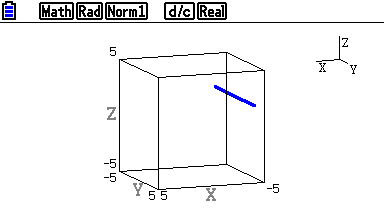
\includegraphics[scale=0.5]{assets/larson11.5q18graph.png}
          \end{center}$\hfill\blacksquare$

    \item The line passes through the point $(2,3,4)$ and is perpendicular to the plane
          given by $3 x+2 y-z=6$. \sol{} The normal vector of the plane is $\vec{n} =
              \langle 3, 2, -1 \rangle$. Hence, the direction vector of the line is $\vec{v}
              = \langle 3, 2, -1 \rangle$. Hence, the parametric equations of the line is
          given by \[x = 2 + 3t \qquad y = 3 + 2t \qquad z = 4 - t\]\\

          \begin{center}
              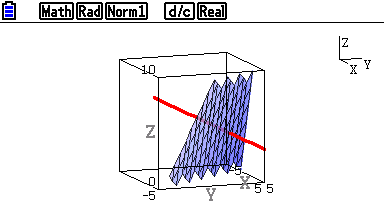
\includegraphics[scale=0.5]{assets/larson11.5q19graph.png}
          \end{center}$\hfill\blacksquare$
\end{enumerate}

\newpage

\begin{enumerate}[label={}, leftmargin=*]
    \item \textbf{Finding a Point of Intersection} In Exercises 33-36, determine whether the lines intersect, and if so, find the point of intersection and the angle between the lines.
\end{enumerate}

\begin{enumerate}
    \setcounter{enumi}{32}
    \item $\begin{aligned}[t] x & =4 t+2, \quad y=3, \quad z=-t+1 \\ x & =2 s+2, \quad y=2 s+3, \quad z=s+1\end{aligned}$

          \sol{} Let the point of intersection be $P(x, y, z)$. Then,
          \begin{align*}
              \langle x, y, z \rangle & = \langle 4t + 2, 3, -t + 1 \rangle = \langle 2s + 2, 2s + 3, s + 1 \rangle
          \end{align*}
          Equating the both sides, we get
          \begin{align*}
              4t + 2 & = 2s + 2 \\
              3      & = 2s + 3 \\
              -t + 1 & = s + 1
          \end{align*}
          Solving the equations, we get $s = 0$ and $t = 0$. Hence, the point of intersection is $P(2, 3, 1)$.

          \begin{align*}
              \cos \theta & = \frac{\vec{v_1} \cdot \vec{v_2}}{\norm{\vec{v_1}} \norm{\vec{v_2}}}                                                           \\
                          & = \frac{\langle 4, 0, -1 \rangle \cdot \langle 2, 2, 1 \rangle}{\norm{\langle 4, 0, -1 \rangle} \norm{\langle 2, 2, 1 \rangle}} \\
                          & = \frac{7}{3\sqrt{17}}                                                                                                          \\
              \theta      & = \arccos \left( \frac{7}{3\sqrt{17}} \right)                                                                                   \\
                          & \approx 55.5^\circ
          \end{align*}$\hfill\blacksquare$\\
          \begin{center}
              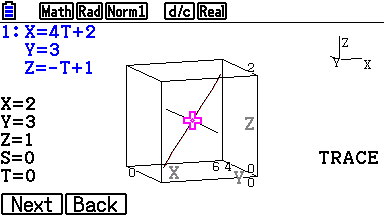
\includegraphics[scale=0.5]{assets/larson11.5q33graph.png}
          \end{center}

          \newpage

          \setcounter{enumi}{34}
    \item $\dfrac{x}{3}=\dfrac{y-2}{-1}=z+1, \quad \dfrac{x-1}{4}=y+2=\dfrac{z+3}{-3}$
          \vspace{0.5cm}
          \begin{multicols}{2}
              \vspace*{-1.3cm}
              \sol{} Let the point of intersection be $P(x, y, z)$. Then,
              \begin{align*}
                  \langle x, y, z \rangle & = \langle 3t, -t + 2, t - 1 \rangle      \\
                                          & = \langle 4s + 1, s - 2, -3s - 3 \rangle
              \end{align*}
              Equating the both sides, we get
              \begin{align*}
                  3t     & = 4s + 1  \\
                  -t + 2 & = s - 2   \\
                  t - 1  & = -3s - 3
              \end{align*}
              Since this system of equations has no solution, the lines do not intersect.$\hfill\blacksquare$\\
              \columnbreak

              \begin{center}
                  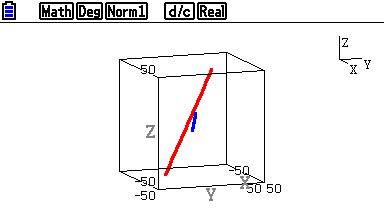
\includegraphics[scale=0.5]{assets/larson11.5q35graph.png}
              \end{center}
          \end{multicols}

    \item $\frac{x-2}{-3}=\frac{y-2}{6}=z-3, \quad \frac{x-3}{2}=y+5=\frac{z+2}{4}$

          \setlength{\columnsep}{1cm}
          \begin{multicols}{2}
              \vspace*{-0.9cm}
              \sol{} Let the point of intersection be $P(x, y, z)$. Then,
              \begin{align*}
                  \langle x, y, z \rangle & = \langle -3t + 2, 6t + 2, t + 3 \rangle \\
                                          & = \langle 2s + 3, s - 5, 4s - 2 \rangle
              \end{align*}
              Equating the both sides, we get
              \begin{align*}
                  -3t + 2 & = 2s + 3 \\
                  6t + 2  & = s - 5  \\
                  t + 3   & = 4s - 2
              \end{align*}
              Solving the equations, we get $s = 1$ and $t = -1$. Hence, the point of intersection is $P(5, -4, 2)$. $\hfill\blacksquare$\\
              \columnbreak

              \begin{center}
                  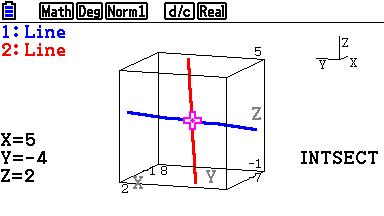
\includegraphics[scale=0.5]{assets/larson11.5q36graph.png}
              \end{center}
          \end{multicols}
\end{enumerate}